% Slides for the Hadwiger--Nelson entry. Every result here also appears in report.tex
% (section given on each slide). Figures are PNG renders of the reader's SVGs
% (slide-figures/, rendered by Edge headless at 2x from HadwigerNelson/Exposition/Figures/).
\documentclass[aspectratio=169,11pt]{beamer}
\usetheme{default}
\setbeamertemplate{navigation symbols}{}
\setbeamertemplate{footline}[frame number]
\usepackage[T1]{fontenc}
\usepackage[utf8]{inputenc}
\usepackage{amsmath,amssymb}
\usepackage{graphicx}
\newcommand{\R}{\mathbb{R}}
\newcommand{\st}[1]{{\footnotesize\textsc{[#1]}}}
\newcommand{\src}[1]{\par\vfill{\scriptsize\color{gray} Report #1}}

\title{Five colours are not enough}
\subtitle{A guided reading of the supplied proof, and two local results about interfaces at a common centre}
\author{[TEAM: names]\\[2pt]{\footnotesize\url{https://github.com/dozenalist/Mathathon}}}
\date{15 November 2026}

\begin{document}
\frame{\titlepage}

\begin{frame}{1. The question}
Colour the plane so that any two points at distance exactly $1$ get different colours. How many colours are needed?
\begin{itemize}
\item $\chi(\R^2)\ge4$: the Moser spindle (1961) \st{cited}
\item $\chi(\R^2)\ge5$: de Grey (2018); Exoo--Ismailescu; Heule \st{cited}
\item $\chi(\R^2)\le7$: a hexagon tiling with seven colours \st{cited}
\end{itemize}
\src{\S1}
\end{frame}

\begin{frame}{2. What was supplied}
\begin{itemize}
\item OpenAI, \emph{The Euclidean plane is not five-colorable} (23 September 2026): every five-colouring has a monochromatic unit pair, so $6\le\chi(\R^2)\le7$. \textbf{Prior work, not ours.} \st{cited}
\item Two moves:
  \begin{enumerate}
  \item a transfer from a proper colouring to a \emph{weak measurable} one (Theorem 1.3);
  \item no weak measurable five-colouring exists (Theorem 1.4).
  \end{enumerate}
\end{itemize}
\src{\S1, \S2}
\end{frame}

\begin{frame}{3. What we did in 40 hours}
\begin{itemize}
\item A six-lesson reader of the second move: refereed, with figures checked by script.
\item A three-centre proof of the manuscript's strict-state separation (Lemma 6.3) \st{proved; Lean 4.34.1}
\item CC60, a closed $60^\circ$ cone obstruction \st{Lean 4.34.1}, and its sharpness above $60^\circ$ \st{proved}
\item Finite computations, negative results and corrections.
\end{itemize}
\medskip
\textbf{No global chromatic result.} The bounds $6\le\chi\le7$ are inherited.
\src{abstract, \S1}
\end{frame}

\begin{frame}{4. Weakness as a ruler experiment}
\begin{columns}[T]
\column{0.48\textwidth}
Drop a unit ruler in a window and turn it at random. It is \emph{bad} if both ends get the same colour.
\smallskip

Weak colouring: the bad share is zero in every window.
\smallskip

Half-plane colouring: half a unit from the boundary, $240^\circ$ of the $360^\circ$ of directions are bad, a share of $2/3$. So it is not weak.
\column{0.5\textwidth}
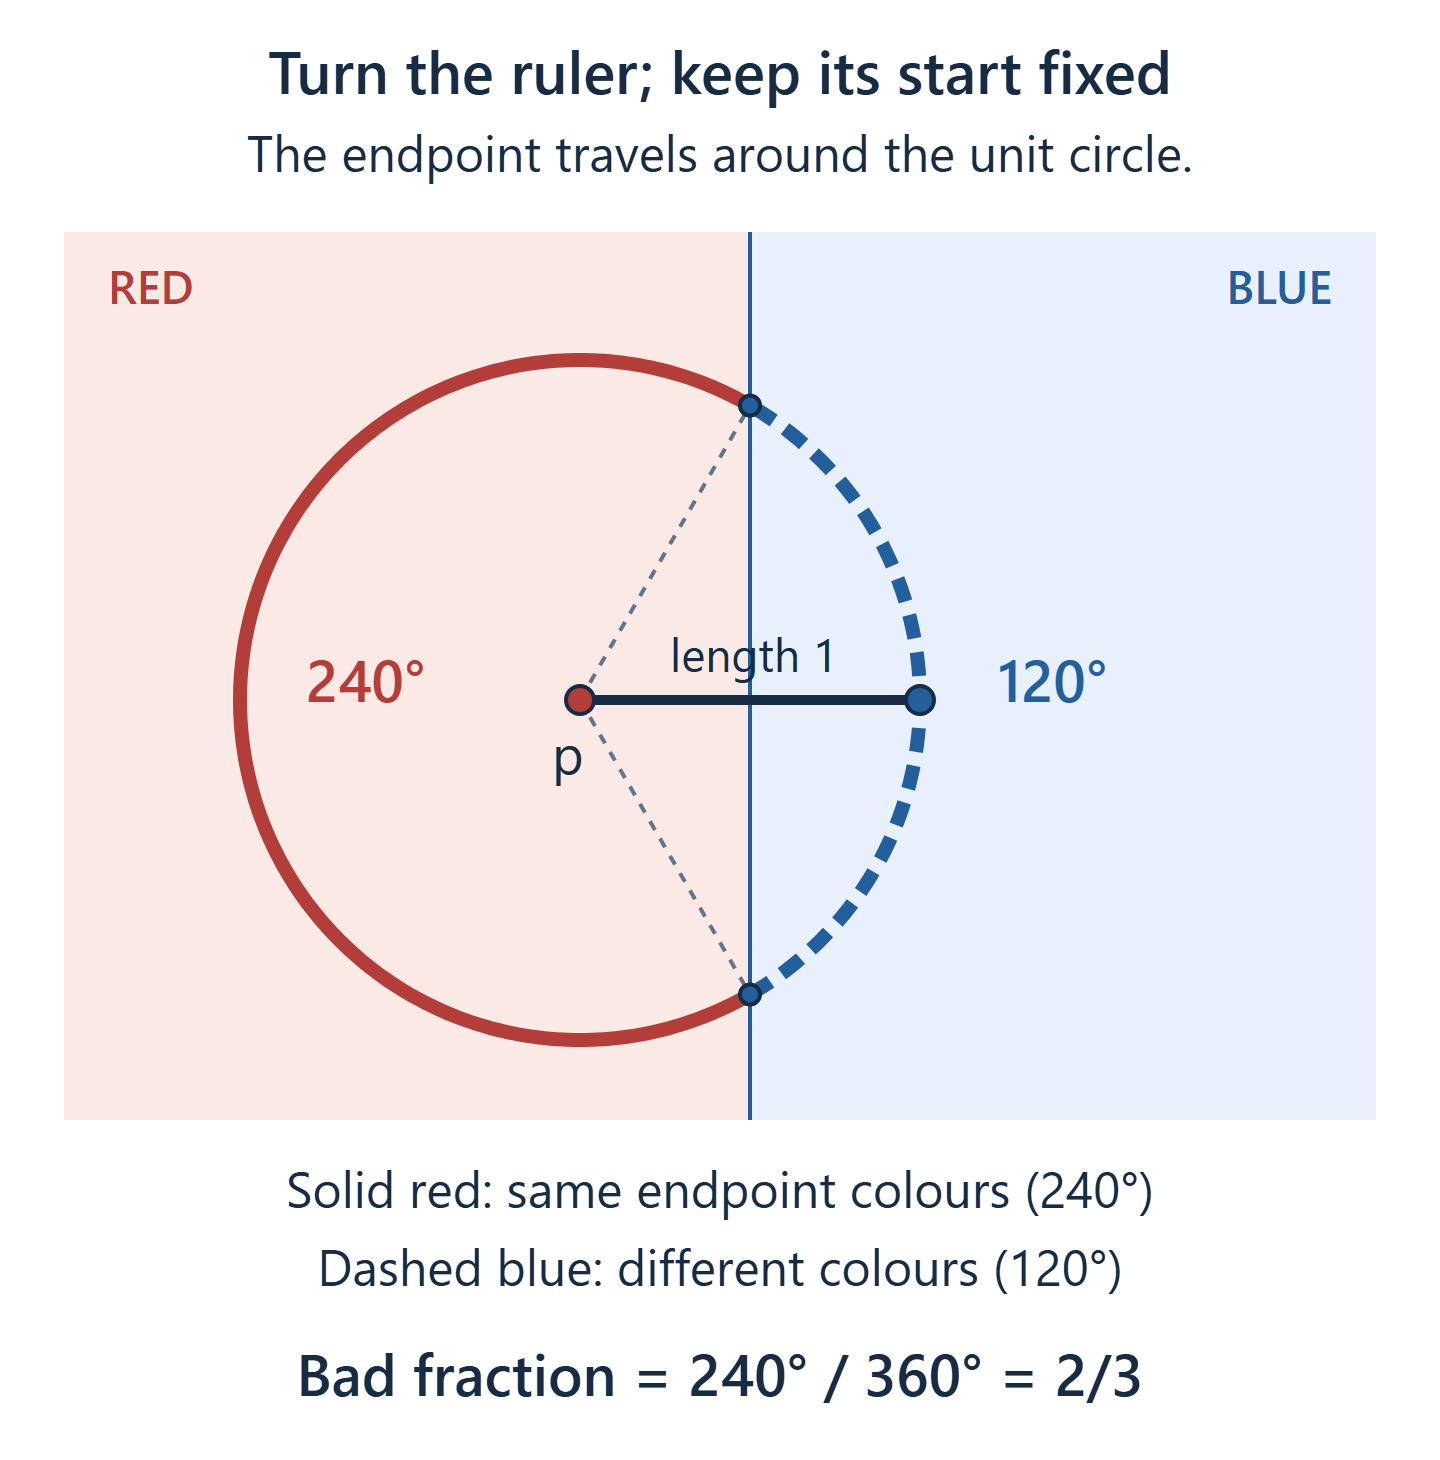
\includegraphics[width=\linewidth,height=0.72\textheight,keepaspectratio]{slide-figures/weak-turning-ruler.png}
\end{columns}
\src{\S2.1, \S6}
\end{frame}

\begin{frame}{5. ``Almost never'' becomes ``never'' (Lemma 4.3)}
\begin{columns}[T]
\column{0.48\textwidth}
Suppose $a$ and $b$, one unit apart, are both robustly inside colour $i$.
\begin{itemize}
\item Start the ruler in $B(a,h)$ and turn it within angle $h$; the tip lands in $B(b,2h)$.
\item The landing disk has $4\times$ the area, so at most $\varepsilon+4\varepsilon$ of starts fail.
\item For $\varepsilon<1/5$ a positive share of rulers is bad, contradicting weakness.
\end{itemize}
\st{cited: manuscript Lemma 4.3}
\column{0.5\textwidth}
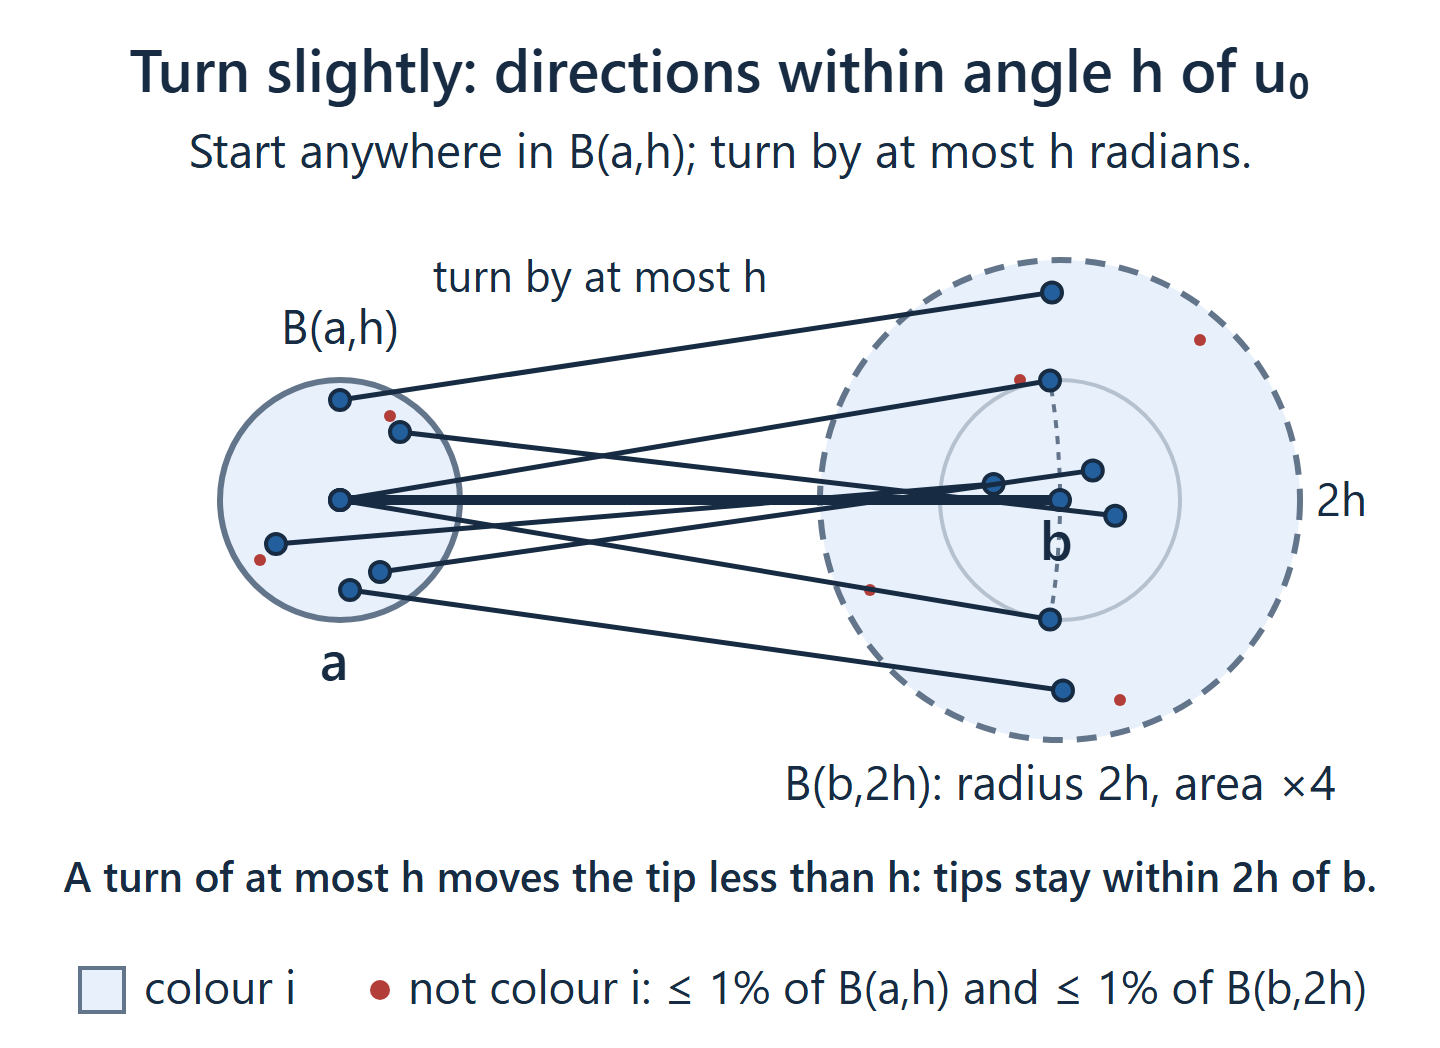
\includegraphics[width=\linewidth,height=0.72\textheight,keepaspectratio]{slide-figures/density-turn.png}
\end{columns}
\src{\S2.2, \S6}
\end{frame}

\begin{frame}{6. Straddling a connected set}
\begin{columns}[T]
\column{0.4\textwidth}
$\Delta(K)=\{z:\min_K|z-q|<1<\max_K|z-q|\}$.
\smallskip

If $K$ is connected, every $z\in\Delta(K)$ is exactly one unit from some point of $K$ (intermediate value theorem).
\smallskip

So a connected set of centres turns one zero-area circle into a band of positive area. Without connectedness the contact can be missing.
\column{0.29\textwidth}
\includegraphics[width=\linewidth]{slide-figures/straddle-band.png}
\column{0.29\textwidth}
\includegraphics[width=\linewidth]{slide-figures/straddle-gap.png}
\end{columns}
\src{\S2.3, \S6}
\end{frame}

\begin{frame}{7. Interfaces at a centre}
\begin{columns}[T]
\column{0.36\textwidth}
Proposition 7.1 builds connected interfaces $K_j$ through a common centre $x$; both labels of a cycle edge occupy zero area of $\Delta(K_j)$.
\smallskip

A tiny interface casts its exclusion on a thin band hugging the unit circle: outside it on the side $K$ points to, inside it on the far side.
\column{0.31\textwidth}
\includegraphics[width=\linewidth]{slide-figures/interface-model.png}
\column{0.31\textwidth}
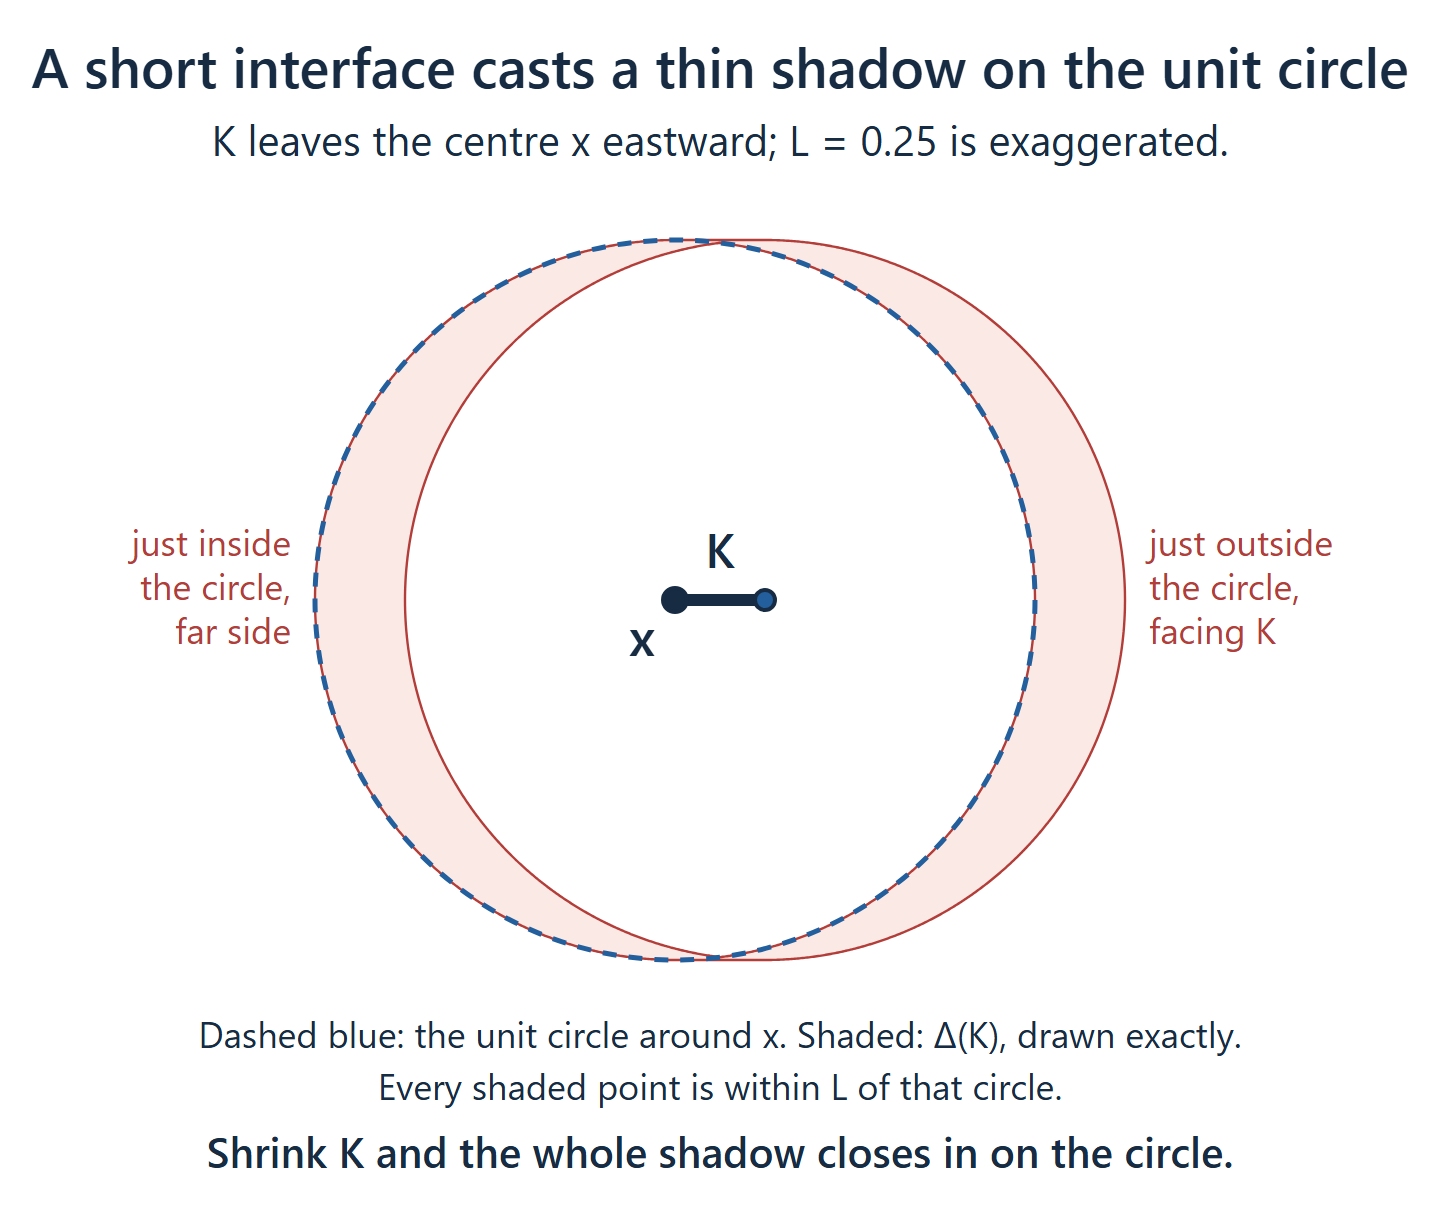
\includegraphics[width=\linewidth]{slide-figures/interface-shadow.png}
\end{columns}
\src{\S2.5, \S6}
\end{frame}

\begin{frame}{8. The proof map}
\begin{columns}[T]
\column{0.55\textwidth}
\footnotesize
\begin{tabular}{@{}ll@{}}
Density & Lemma 4.3\\
Palettes & Def.~5.1, Remark 5.3, Cor.~5.4\\
Two labels & Lemma 5.5, Prop.~5.6\\
States & Lemmas 6.2--6.4, Thm 6.5\\
Interfaces & Prop.~7.1\\
Strips & Lemma 8.1\\
Cycles & Props 8.2, 8.5, 8.10 (Moser spindle)
\end{tabular}
\smallskip

\normalsize Step 5 has exactly three branches, and each ends in a contradiction.
\column{0.43\textwidth}
\includegraphics[width=\linewidth,height=0.72\textheight,keepaspectratio]{slide-figures/proof-casefan.png}
\end{columns}
\src{\S2.6}
\end{frame}

\begin{frame}{9. Three centres, one leftover label}
\begin{columns}[T]
\column{0.4\textwidth}
\footnotesize
\textbf{Theorem.} If $(A,J)$ and $(B,K)$ are states at $x$, $|A|>0$, and $X$ is the only label outside $J\cup K$, then no two support directions of $B$ are $60^\circ$ apart.
\smallskip

\textbf{Proof.} $x$, $y=x+e^{ib}$ and $z=x+e^{id}$ are mutually one unit apart, so their palettes are disjoint. $P_y$ and $P_z$ are not inside $K$, and $J\subseteq P_x$. Each of $P_y$, $P_z$ must contain $X$: contradiction.
\smallskip

\st{proved; Lean 4.34.1; integrated in the team build R1}
\column{0.29\textwidth}
\includegraphics[width=\linewidth]{slide-figures/three-centre-triangle.png}
\column{0.29\textwidth}
\includegraphics[width=\linewidth]{slide-figures/three-centre-count.png}
\end{columns}
\src{\S3}
\end{frame}

\begin{frame}{10. CC60: a closed $60^\circ$ cone}
\begin{columns}[T]
\column{0.5\textwidth}
\footnotesize
Weak measurable colouring with any finite number of labels; finitely many sets $K_i\ni x$ approaching $x$ from signed directions $v_i$, all in one \emph{closed} $60^\circ$ arc; each label of $F_i$ occupies zero area of $\Delta(K_i)$.
\smallskip

\textbf{Then at least three labels lie outside every $F_i$.}
\smallskip

Sets need not be connected or compact. Equality at $60^\circ$ is included.
\smallskip

\st{proved, refereed; Lean 4.34.1: \texttt{closed60\_exclusions\_three\_le}}
\column{0.48\textwidth}
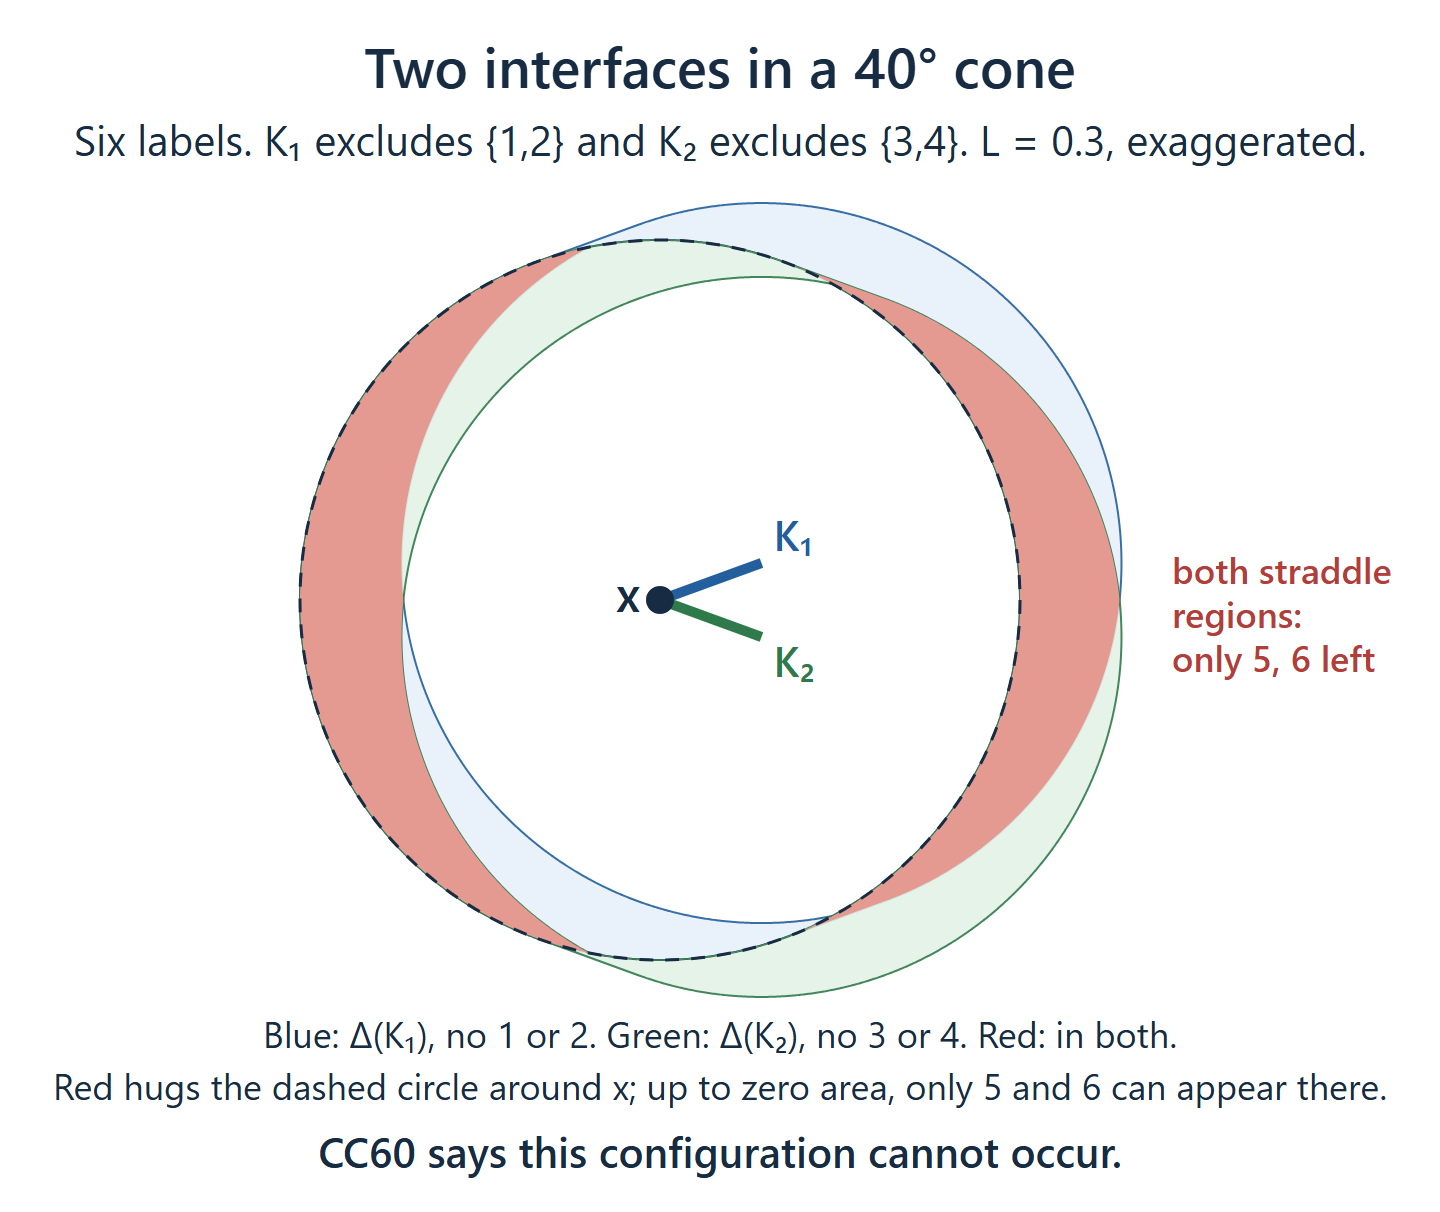
\includegraphics[width=\linewidth,height=0.7\textheight,keepaspectratio]{slide-figures/interface-cone.png}
\end{columns}
\src{\S4}
\end{frame}

\begin{frame}{11. Sharpness and limits of CC60}
\begin{itemize}
\item For every cone wider than $60^\circ$, a Borel, pointwise proper 20-colouring with two segment interfaces leaves only two labels. So CC60 cannot be widened for arbitrary finite palettes. \st{proved, refereed; not Lean}
\item Six-colour sharpness and novelty priority are \textbf{not} established.
\item CC60 forbids a kind of local configuration. Nothing shows that a six-colouring must produce it.
\end{itemize}
\src{\S4}
\end{frame}

\begin{frame}{12. Further local results}
\begin{itemize}
\item \textbf{Canonical paired palette excluded.} In a weak measurable six-colouring, no centre has a palette containing the canonical paired palette $P(t)$ for almost every $t$. The reason is a finite unit-distance configuration with no proper list colouring. \st{proved, refereed}
\item \textbf{Even walks.} In an open set where every point of a connected piece has a unit neighbour, any two points are joined by an even unit walk. This gives finite list and parity obstructions for weak measurable $k$-colourings. \st{Lean 4.34.1}
\item \textbf{Six-colour producer pieces.} Each piece compiles, but the glued statement still assumes two hypotheses (SignTable, ForcingLemma). \st{Lean 4.34.1, conditional}
\item None of these is a global chromatic result. The open lemmas behind a route to $\chi\ge7$ are listed in the report.
\end{itemize}
\src{\S5}
\end{frame}

\begin{frame}{13. Computations and corrections}
\begin{itemize}
\item Exact certificates for a translated union of Heule graphs (1,048 vertices) and for no forced-equal pairs \st{computation}
\item Direction filtering on a grid: 7,776 $\to$ 1,420 $\to$ 174 $\to$ 6 (an earlier count of 95 was a bug) \st{computation}
\item The closed-$120^\circ$ ``monochromatic'' endpoint claim is false: a refereed 19-colour counterexample \st{proved}
\item Simplification of the supplied Lean proof: 150 lines shorter in the team build (126 from the encoding refactor, 24 net from R1) \st{Lean 4.34.1}
\end{itemize}
\src{\S5}
\end{frame}

\begin{frame}{14. Honest status}
\begin{itemize}
\item \textbf{No global chromatic result.} $6\le\chi(\R^2)\le7$ is unchanged.
\item Lean checks ran under 4.34.1; the event's Lean track needs 4.35.0, which has not been rebuilt.
\item AI use: Claude drafted and refereed the exposition and this report. Research workers did the reviews and Lean work. Every claim was checked against the sources, the logs or exact scripts.
\item Ask us about the definitions, the key step, what is new versus cited, and how sure we are.
\end{itemize}
\src{\S7--\S10}
\end{frame}
\end{document}
